% GENERATED by paper/tex/build_uk.py from paper/article-ua.txt. Do not edit by hand.
\documentclass[11pt]{article}
\newcommand{\tablelang}{uk}
% Shared preamble for paper/tex/en/main.tex and paper/tex/uk/main.tex (XeLaTeX via Tectonic).
% Same layout as the author's earlier preprint (Zenodo 23375871): A4, 25 mm, CMU fonts, natbib numbers.
\usepackage[a4paper,margin=25mm]{geometry}
\usepackage{fontspec}
\setmainfont{cmunrm.otf}[BoldFont=cmunbx.otf,ItalicFont=cmunti.otf,BoldItalicFont=cmunbi.otf]
\setsansfont{cmunss.otf}[BoldFont=cmunsx.otf,ItalicFont=cmunsi.otf]
\setmonofont{cmuntt.otf}[BoldFont=cmuntb.otf,ItalicFont=cmunit.otf]
\usepackage[ukrainian,english]{babel}
\usepackage{amsmath,amssymb}
\usepackage{booktabs,tabularx,array,longtable}
\usepackage{graphicx}
\usepackage[font=small,labelfont=bf]{caption}
\usepackage{xcolor}
\usepackage{microtype}
\usepackage[numbers,sort&compress]{natbib}
\PassOptionsToPackage{hyphens}{url}
\usepackage[hidelinks]{hyperref}
\usepackage[nameinlink,capitalise,noabbrev]{cleveref}
\usepackage{url}

\graphicspath{{../../figures/}}
% primitive input: LaTeX's \input is not expandable and breaks inside tabular after \midrule
\makeatletter\newcommand{\gentable}[1]{\@@input ../tables/\tablelang/T#1.tex }\makeatother
\newcommand{\code}[1]{\texttt{#1}}
\newcolumntype{L}{>{\raggedright\arraybackslash}X}
\newcolumntype{R}{>{\raggedleft\arraybackslash}p{1.1cm}}
\definecolor{lvA}{HTML}{2a78d6}\definecolor{lvB}{HTML}{eb6834}\definecolor{lvC}{HTML}{1baf7a}\definecolor{lvD}{HTML}{eda100}
\setlength{\tabcolsep}{4pt}
\renewcommand{\arraystretch}{1.12}
\setlength{\emergencystretch}{2em}
\sloppy

\addto\captionsukrainian{\renewcommand{\refname}{Література}}
\hypersetup{pdftitle={Дешеві агенти-програмісти у виживанні Minecraft},pdfauthor={Олександр Пилипенко}}
\begin{document}
\selectlanguage{ukrainian}
\title{Дешеві агенти-програмісти у виживанні Minecraft: перевірена бібліотека навичок, дванадцятиденний прогін чотирьох агентів Gemini~3.8~Flash і аудит кожної віхи за логом сервера}
\author{Олександр Пилипенко\\[2pt]\small ORCID 0009-0004-9610-9242}
\date{2026-11-02 \quad (v1.0)}
\maketitle
\begin{abstract}
\noindent
Ми відтворили частину постановки препринту arXiv:2610.22319, де четверо агентів Gemini 4 Argon пройшли Minecraft, керуючи гравцями лише через JavaScript-програми для бібліотеки Mineflayer. Відмінності нашої постановки: дешевша модель (Gemini 3.8 Flash High через Antigravity CLI), обмежений бюджет токенів і перевірена бібліотека навичок, яку агенти отримують на старті. Бібліотека містить 54 функції, зокрема рекурсивне lib.obtain(item, n), що з даних гри виводить увесь ланцюжок передумов. Ми описуємо інфраструктуру (міст із пісочницею, сторож ходів, <<паркування>> бота без агента, огляд розрізом), 20 дефектів, знайдених під час її тестування, два пілотні прогони й основний прогін тривалістю 294 календарні години, з яких 20,1 години активної гри. За цей час 2–4 агенти виконали 3770 програм (21,2\% завершилися помилкою, 70,4\% помилок — таймаути) і загинули 332 рази. Головний внесок — аудит: кожна з 16 віх отримує рівень доказовості A–D за формальним правилом, що читає лог сервера. Рівень A означає, що до віхи на сервері не було жодної консольної команди. Етап 1 (камінь, залізо, броня, ліжко, алмази, алмазна кирка, кресало, обсидіан) агенти пройшли на рівні A за 2,4 активної години. Вхід у Незер, фортеця й перший стрижень іфрита мають рівень B (допомога — лише пропуск ночі), але на той момент агенти вже користувалися хелперами, які під час прогону додала керівна сесія оператора (позначка +K). Перли й Око Енду мають рівень C (тривалі ефекти, зачарування, keepInventory). Стронгхолд, Енд і дракона ми не зараховуємо агентам: ці віхи виконали консольні команди (телепорт, /fill порталу, урон дракону, видача досягнення) — рівень D. 63,6\% смертей припадають на вогонь, вогняні кулі гастів і лаву. Модель витратила 13 652 кроки, 50,8 млн незакешованих вхідних токенів (ще 1922,9 млн з кешу, 97,4\%), 8,82 млн вихідних і 4,06 млн токенів міркування.
\end{abstract}

\medskip\noindent\textbf{Ключові слова.} LLM-агенти; багатоагентні системи; Minecraft; Mineflayer; бібліотека навичок; довгий горизонт; аудит; відтворюваність.

\medskip\noindent\textbf{Заява про незалежність.} Це незалежне часткове відтворення постановки arXiv:2610.22319 (Google DeepMind). Станом на 2026-11-02 контакту з авторами не було; роботу не узгоджено з ними й не рецензовано ними. Ми не використовуємо Gemini 4 Argon і не стверджуємо, що наші результати порівнянні з їхніми напряму.

\medskip\noindent\textbf{Заява про використання ШІ.} Інфраструктуру, бібліотеку навичок, гайди для агентів, скрипти аналізу й чернетку тексту створено в сесіях Claude Code (Claude Opus 5.5, Anthropic) під керівництвом автора. Гравцями керували агенти Gemini 3.8 Flash High через Antigravity CLI (agy). Окрема сесія agy (далі — керівна сесія) виконувала запити автора під час прогону: запускала й зупиняла гру, редагувала інструкції та хелпери агентів і, на прохання автора, виконувала консольні команди сервера. Ілюстрацію для README згенеровано моделлю зображень Gemini. Усі числа статті автор може перевірити запуском scripts/run\_all.sh на опублікованих даних.

\section{Вступ і мотивація}

У препринті arXiv:2610.22319 четверо агентів Gemini 4 Argon за 27 год 14 хв пройшли Minecraft від голих рук до перемоги над драконом Енду, виконавши 2783 програми й загинувши 605 разів. Агенти не мали жодних інструментів, специфічних для гри: лише Mineflayer, плагін пошуку шляху й один абзац мети. Вартість прогону автори оцінюють приблизно в 520 доларів за вступною ціною.

Інший полюс — Odyssey (arXiv:2407.15325): велика бібліотека навичок (40 примітивних і 183 складені) дозволяє навіть 8-мільярдній моделі виконувати задачі на кшталт <<отримати алмаз>>. Без бібліотеки, за абляцією авторів, така модель майже не генерує виконуваного коду.

Нас цікавило проміжне питання: як далеко зайдуть дешевші агенти-програмісти, якщо дати їм перевірену бібліотеку навичок і гайди, але залишити повну свободу коду й координації, і як чесно звітувати про прогін, у який під тиском бюджету втручався оператор. Друге питання виявилося не менш важливим за перше: у нашому прогоні керівна сесія оператора на його прохання наприкінці <<довела>> гру консольними командами, і без аудиту за логом сервера ця частина виглядала б як результат агентів.

\section{Що перевіряється і що поза межами}

Перевіряється:
\begin{itemize}
\item наскільки далеко по дереву технологій Minecraft доходять 2–4 агенти Gemini 3.8 Flash High із бібліотекою навичок, сторожем і гайдами, і за який активний час;
\item які збої (смерті, помилки програм, дефекти інфраструктури) визначають темп;
\item чи можна механічно, за логом сервера, відокремити досягнуте агентами від зробленого командами оператора.
\end{itemize}

Поза межами:
\begin{itemize}
\item порівняння моделей у контрольованих умовах (у нас один прогін і одна модель);
\item перемога над драконом агентами (не досягнута, див. розд. 6.2);
\item гра з пікселів: агенти бачать світ лише через API Mineflayer;
\item оцінка якості самих гайдів окремо від бібліотеки (вони змінювалися разом).
\end{itemize}

\section{Внески (і чого вони не стверджують)}

\begin{enumerate}\renewcommand{\labelenumi}{(\alph{enumi})}
\item Відкрита інфраструктура: міст до Mineflayer із пісочницею vm і списком дозволених модулів, CLI ./mc для агентів, сторож ходів agy, <<паркування>> бота без агента, захист поставлених блоків від pathfinder, огляд зверху з розрізом. Не стверджуємо, що вона оптимальна чи переноситься на інші версії гри без змін.
\item Бібліотека навичок із 54 функцій, зокрема lib.obtain, що виводить ланцюжок передумов із даних гри (рецепти, дропи блоків, інструменти, плавка, дроп мобів). Кожну навичку перевірено на сервері; знайдені дефекти перелічено в табл. 7. Не стверджуємо повноти: бій, Незер і Енд бібліотека покриває слабко.
\item Результати двох пілотів і основного прогону з рівнями доказовості A–D для 16 віх (табл. 2). Не стверджуємо, що агенти пройшли гру: віхи M14–M16 мають рівень D.
\item Метод аудиту: формальне правило за логом сервера й окрема позначка +K для хелперів, доданих оператором під час прогону. Не стверджуємо, що він виявляє всі форми допомоги: зміни інструкцій і порад агентам він бачить лише через використання хелперів.
\item Аналіз збоїв: 332 смерті за причинами й фазами, 798 невдалих програм за класами. Не стверджуємо причинно-наслідкових зв'язків між фазою допомоги й смертністю: фази збігаються з переходом у Незер.
\item Облік вартості в токенах для основного прогону. Не стверджуємо грошової вартості: квотований доступ через Antigravity не має прозорої ціни за токен.
\end{enumerate}

\section{Середовище і агенти}

\subsection{Сервер}
Vanilla Minecraft Java Edition 1.20.1 у Docker (образ itzg/minecraft-server), виживання, складність Easy, без читів, командних блоків і RCON; оператором є лише людина-спостерігач. Спершу ми використовували 1.20.4, як у arXiv:2610.22319, але перейшли на 1.20.1, бо 3D-переглядач prismarine-viewer має палітру станів блоків саме цієї версії, а на 1.20.4 малював підземні блоки неправильно (дефект D12).


\subsection{Міст}
Для кожного гравця працює окремий процес Node.js із ботом Mineflayer. Агент пише програму у файл і запускає ./mc run файл --timeout N. Програма виконується як тіло async-функції в пісочниці vm; глобальні змінні: bot, lib, console, isCancelled(), Vec3, mcData, goals, Movements, sleep. Дозволено require лише пакетів Mineflayer і кількох нешкідливих модулів Node; процеси, файли й мережа недоступні. Значення в globalThis зберігаються між програмами, а файли autoload.js команди й агента виконуються після кожного старту моста. Після таймауту програма отримує isCancelled() = true, а рух і копання зупиняються. Вивід програми доповнюється позицією, здоров'ям, їжею, фазою доби, ворогами поруч, міцністю інструментів і новим чатом. Якщо 5 хвилин немає програм, бот виходить із гри (<<паркування>>) і повертається з наступною програмою; чат і події за цей час міст читає з лога сервера.


\subsection{Бібліотека навичок}
54 функції (bridge/lib/skills.js і obtain.js, разом 1442 рядки на кінець прогону): огляд світу, рух (з копанням, але без руйнування поставлених агентами блоків), збір, крафт із відновленням після збоїв, ставлення блоків і креслення (будинок, рамка порталу), скрині, плавка, бій, укриття, сон, спуск сходами до алмазів, відро, обсидіан із лави й води, двері. Центральна навичка lib.obtain(item, n) рекурсивно обирає між плавкою, крафтом, полюванням і копанням, сама добуває потрібний інструмент і паливо, повторює спроби й зупиняється після смерті гравця. У тестах з порожнього інвентарю залізна кирка вийшла за 96 с, відро за 99 с, повна залізна броня приблизно за 6 хв.


\subsection{Інструкції}
AGENTS.md (мета, золоті правила, як грати, пам'ять) і сім гайдів (бібліотека, виживання, програми й помилки, рецепти, будівництво, командна робота, залізний вік) — разом 7452 слова. Гайди писалися з досвіду пілотів і тестів; кожен шматок коду в них перевірено на сервері.


\subsection{Агенти}
Кожного гравця веде окремий агент Gemini 3.8 Flash High в Antigravity CLI з дозволом на всі інструменти. Сторож (agent-loop.sh) запускає хід за ходом у тій самій розмові й після кожного ходу додає свіжий статус гравця. До 24.10 грали двоє (alpha, beta), далі четверо (gamma, delta приєдналися 24.10 о 17:22 UTC). Мета в інструкціях: дракон Енду як довга ціль і поточний етап із пронумерованими віхами.


\subsection{Огляд}
Для спостереження ми написали камеру, що стежить за гравцем згори, а під землею показує розріз (блоки над гравцем не малюються), і затемнення неба за ігровим часом (D13, D14). Агенти огляду не бачать.


\subsection{Як lib.obtain виводить ланцюжок}
Виклик lib.obtain(item, n) гарантує, що в інвентарі є щонайменше n предметів, і для кожного відсутнього предмета обирає джерело в такому порядку. (1) Плавка, якщо предмет є в таблиці плавки (злитки, скло, приготоване м'ясо, деревне вугілля): навичка спершу добуває вхідний матеріал, потім паливо з розрахунку 8 предметів на одиницю вугілля або 1,5 на дошку чи колоду, і лише тоді, перед самою плавкою, шукає або ставить піч. (2) Крафт: серед усіх рецептів обирається найдешевший за оцінкою вартості інгредієнтів; рецепти, що споживають блоки-сховища (iron\_block, nugget), відкидаються, а рецепти з тієї самої родини предметів (ліжко з ліжка, вовна з вовни) отримують штраф 5000, щоб уникнути циклів перефарбування. Верстак готується першим, бо інакше він <<з'їдає>> дошки, зібрані для рецепта; інгредієнти добираються кількома проходами, доки не будуть в інвентарі одночасно. (3) Полювання для предметів, що випадають із мобів (шкіра, вовна, нитки, перли). (4) Копання: блоки-джерела береться з даних гри (drops), потрібний інструмент — з harvestTools; якщо його немає, навичка рекурсивно добуває найдешевший придатний. Для глибоких руд, яких немає поруч, навичка спершу спускається сходами на типовий рівень руди (алмази −54) з трьома запасними кам'яними кирками, а якщо сходи впираються в рідину, відходить на \textasciitilde{}28 блоків і починає знову. Обсидіан, якого майже ніколи немає готового, навичка робить сама: виливає воду на край лавового озера й копає алмазною киркою. Кожен крок записується в журнал, який повертається агенту; якщо гравець гине, навичка негайно зупиняється й повідомляє, де лежать речі.


\section{Метод аудиту}

Джерело правди — лог сервера Minecraft. Скрипт extract.py розбирає всі файли лога в таблицю подій: досягнення, смерті, входи й виходи, чат і зворотний зв'язок консольних команд. Рядки на кшталт <<Teleported …>>, <<Applied effect …>>, <<Successfully filled …>> не мають імені гравця; у нашій конфігурації оператором є лише людина-спостерігач, тому такі рядки походять від консолі сервера, яку керівна сесія використовувала через docker exec.

Рівень віхи визначається за командами, що з'явилися в основному прогоні до неї:

A — жодної консольної команди;

B — лише перемотування часу й правило playersSleepingPercentage (пропуск ночі), а також запити лише для читання;

C — уже діяли підсилення: ефекти, зачарування, ігрові правила (keepInventory), видача предметів, заповнення блоків;

D — за 15 хвилин до віхи був телепорт, урон, знищення сутностей, видача предмета чи досягнення.

Окремо: +K, якщо агенти вже використали хелпери, які керівна сесія додала в team/autoload.js під час прогону (табл. 2, останній стовпчик). Перше використання береться з коду програм. Ми не змогли приписати визначення цих хелперів жодному запису самих агентів.

Початок основного прогону — 2026-10-21 12:11 UTC, запуск агентів. Програми о 12:06–12:10 були нашими тестами бібліотеки на тому самому гравці alpha: вони дали alpha кам'яну й залізну кирки до старту (див. розд. 8). Тому віхи M01 і M02 зараховано beta, яка дійшла до них сама.

Покриття: 3766 із 3770 програм основного прогону припадають на інтервали, для яких лог сервера існує; решта 4 — секунди зупинки сервера. Лог за 2026-10-21 00:00–11:59 UTC втрачено (ротація при перезапусках); це стосується лише ночі простою після пілоту 2, яку ми рахуємо за логом моста.

Активний час — сума інтервалів виконання програм усіх агентів, де проміжки до 5 хвилин вважаються грою (агент думає); довші паузи (квота, зупинки) не враховуються.

\section{Результати}

\subsection{Пілоти}
Пілот 1 — двоє агентів без гайдів і без бібліотеки, мета <<збудувати споруду>>. За 15 хвилин — 8 смертей уночі (34,9 на активну годину) і близько 20 блоків стін, після чого автор зупинив прогін. Пілот 2 — з гайдами й першою версією бібліотеки: 2 смерті за активну гру, будинок 5×5 із пісковику (89 блоків, обидва агенти незалежно перевірили його через lib.materials) і агенти, що, оголосивши <<100\% COMPLETE>>, завершили хід. Боти без агентів простояли 8,2 години ночі й загинули 42 рази; від будинку лишилося близько 60 із 89 блоків, найімовірніше через вибухи кріперів. Ці два спостереження дали сторожа ходів (D15) і паркування (D16).

\begin{table}[h]\centering\small
\caption{Прогони. Активні години — об'єднання інтервалів програм із проміжками до 5 хв; lib\,\% — частка програм, що викликають бібліотеку.}\label{tab:T1}
\begin{tabularx}{\linewidth}{@{}L rrrrrrr@{}}\toprule
прогін & агентів & год календ. & год активн. & програм & помилки \% & смерті & lib \% \\\midrule
\gentable{1}\bottomrule\end{tabularx}
\end{table}


\subsection{Основний прогін: віхи}
Табл. 2 і рис. 1. Етап 1 агенти пройшли на рівні A без хелперів оператора: перші кам'яні інструменти beta отримала за 2 хвилини після старту, алмази й алмазну кирку — за 2,0–2,1 активної години, обсидіан (вода на лаву) — за 2,4. Вхід у Незер (delta, 7,4 активної години), фортецю (delta, 9,6) і стрижень іфрита (gamma, 13,4) досягнуто на рівні B, тобто без консольної допомоги, крім пропуску ночі, але з +K: агенти вже використовували хелпери оператора, зокрема makeObsidianSafe для обсидіану порталу й configureFireAvoidance для обходу вогню. Перли Енду й Око Енду (beta, 18,9 і 19,1) — рівень C: на той момент діяли нескінченні ефекти (Haste III, Resistance, Fire Resistance, Speed, Saturation), зачарування Looting III і keepInventory. Кімнату порталу в стронгхолді, вхід в Енд і смерть дракона за 5 хвилин (18:01–18:06 UTC 2 листопада) ми агентам не зараховуємо: керівна сесія знайшла стронгхолд, читаючи файли регіонів світу, заповнила портал блоками end\_portal, телепортувала гравців, знищила кристали, завдала дракону урону командами /damage і видала досягнення командою /advancement — рівень D.

\begin{table}[h]\centering\small
\caption{Віхи основного прогону: коли будь-який агент досяг кожної вперше, рівень доказовості й кількість хелперів оператора вже у вжитку (+K).}\label{tab:T2}
\begin{tabularx}{\linewidth}{@{}l L l l r r c r@{}}\toprule
id & віха & вперше (UTC) & агент & год календ. & год активн. & рівень & хелпери опер. \\\midrule
\gentable{2}\bottomrule\end{tabularx}
\end{table}

\begin{figure}[h]\centering
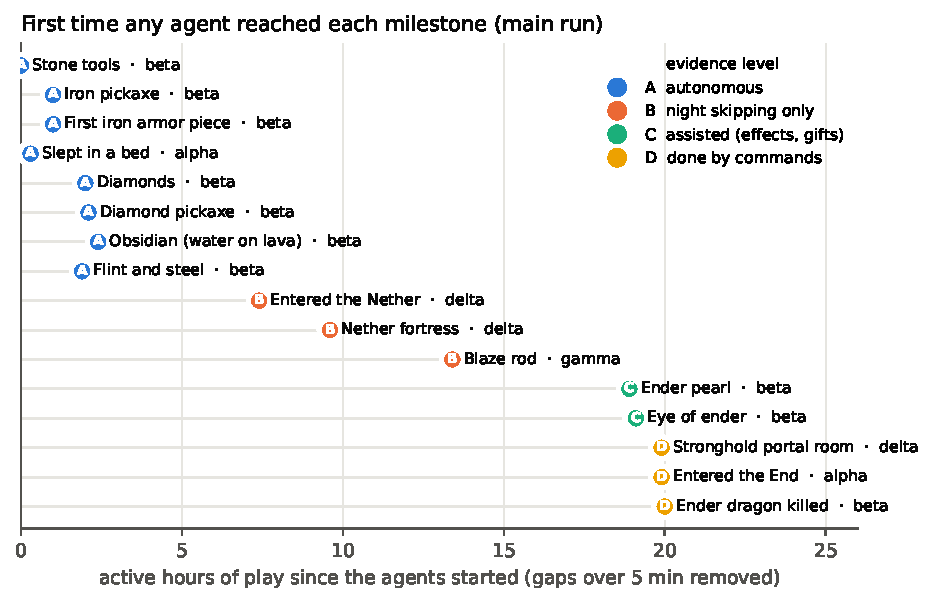
\includegraphics[width=1.0\linewidth]{F1_timeline.pdf}
\caption{Коли будь-який агент уперше досяг кожної віхи, за активними годинами; колір і літера — рівень доказовості.}
\end{figure}

\subsection{Втручання}
Табл. 3 і рис. 3. У фазі A консольних команд не було. У фазі B (з 23.10) — лише 59 команд часу й сну (time set, playersSleepingPercentage) та 8 запитів досвіду. Фаза C почалася 1.11 о 17:00 UTC: після запиту автора на <<всі покращення>> (31.10) керівна сесія розширила скрипт auto-skip-night.sh, і він через консоль увімкнув keepInventory, ефекти й зачарування. Фазу D автор запустив 2.11 о 17:59 словами <<це вже не робота агентів, це тупий фарм… їм треба допомагати максимально>>. Склад команд у фазі C: 702 заповнення блоків (здебільшого відновлення рамки порталу кожні 15 с), 55 ефектів, 26 зачарувань, 20 ігрових правил, 15 точок відродження, 2 видачі предметів. Фаза D тривала 12 хвилин і містила 15 телепортів, 100 заповнень блоків (портал Енду, доріжки в Енді), 5 команд урону, 1 знищення сутностей, 3 видачі предметів і 2 видачі досягнень. Разом 1071 консольна команда.

\begin{table}[h]\centering\small
\caption{Консольні команди основного прогону за родинами й фазами.}\label{tab:T3}
\begin{tabularx}{\linewidth}{@{}L rrrrr@{}}\toprule
родина & A & B & C & D & разом \\\midrule
\gentable{3}\bottomrule\end{tabularx}
\end{table}

\begin{figure}[h]\centering
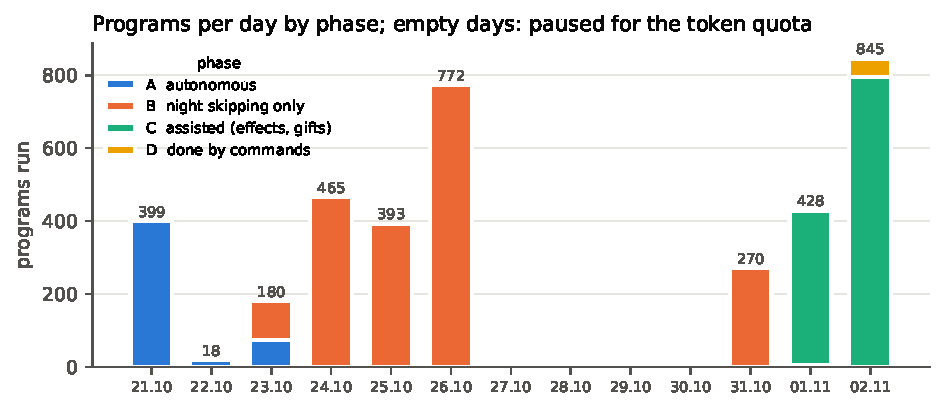
\includegraphics[width=1.0\linewidth]{F3_activity.pdf}
\caption{Програми за день за фазами. Дні без стовпчиків: гру зупинено через квоту токенів.}
\end{figure}

\subsection{Смерті}
Табл. 4, рис. 2 і 4. З 332 смертей основного прогону 211 (63,6\%) припадають на вогонь, вогняні кулі гастів і лаву, тобто на Незер. У фазі A — 11 смертей за 4,5 активної години (2,4 на годину, головна причина — утоплення), у фазі B — 17,7 на годину, у фазі C — 25,1. Зростання збігається з переходом у Незер, а не лише з фазою допомоги; навіть з Fire Resistance фаза C дала 48 смертей від вогню, бо агенти без обережності ходили по полю душ і біля лави.

\begin{table}[h]\centering\small
\caption{Смерті основного прогону за причинами й фазами.}\label{tab:T4}
\begin{tabularx}{\linewidth}{@{}L rrrrr@{}}\toprule
причина & A & B & C & D & разом \\\midrule
\gentable{4}\bottomrule\end{tabularx}
\end{table}

\begin{figure}[h]\centering
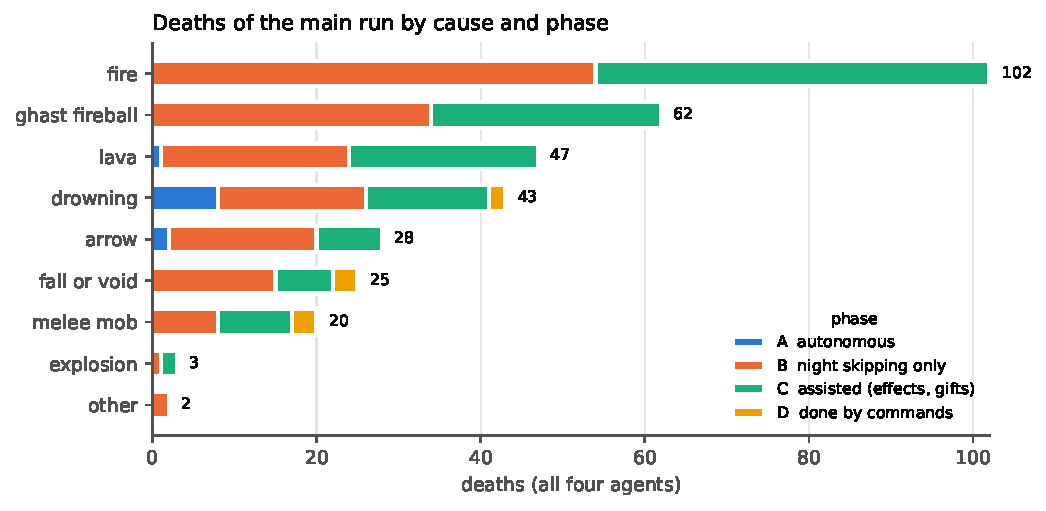
\includegraphics[width=1.0\linewidth]{F2_deaths.pdf}
\caption{Смерті основного прогону за причинами, з розподілом за фазами.}
\end{figure}
\begin{figure}[h]\centering
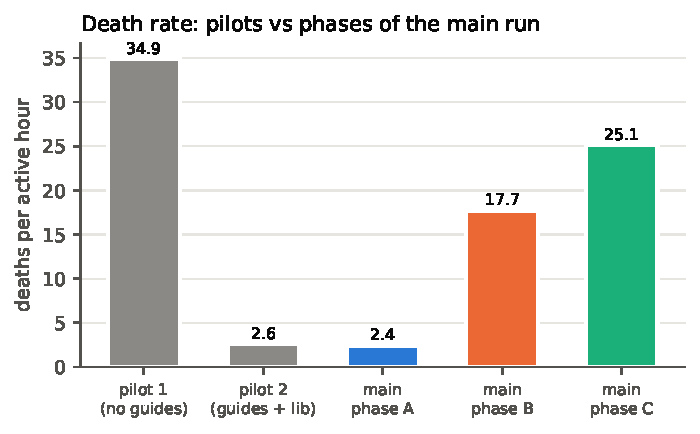
\includegraphics[width=0.72\linewidth]{F4_death_rate.pdf}
\caption{Смерті на активну годину в пілотах і фазах основного прогону (фаза D тривала 12 хвилин і не показана).}
\end{figure}

\subsection{Помилки програм}
Табл. 5. 798 із 3770 програм (21,2\%) завершилися помилкою; 70,4\% із них — таймаути, коли агент обрав замалий час для тривалої дії (видобуток, марш у Незері). Помилки самого коду (TypeError, ReferenceError) становлять лише 4,0\% невдалих програм: модель упевнено пише JavaScript, а слабке місце — оцінка тривалості дій і ситуацій у світі.

\begin{table}[h]\centering\small
\caption{Програми з помилкою в основному прогоні за класами.}\label{tab:T5}
\begin{tabularx}{\linewidth}{@{}L rr@{}}\toprule
клас & програм & \% від невдалих \\\midrule
\gentable{5}\bottomrule\end{tabularx}
\end{table}


\subsection{Агенти й вартість}
Табл. 6. Медіанна програма триває 8,8 с. Частка програм із lib.obtain невелика (1,2–3,7\%), бо агенти загортали її у власні хелпери; бібліотеку загалом використовують 92,6\% програм. Токени облічено за власним потоком кожного агента (крок моделі = відповідь або виклик інструмента): 13 652 кроки, 50,8 млн незакешованих вхідних токенів, 1922,9 млн закешованих (97,4\%), 8,82 млн вихідних і 4,06 млн токенів міркування. Квота Antigravity змушувала зупиняти гру: 27–30.10 гра стояла повністю (рис. 3).

\begin{table}[h]\centering\footnotesize
\caption{Агенти основного прогону. Стовпці токенів — у мільйонах; кеш — вхідні токени з кешу контексту.}\label{tab:T6}
\setlength{\tabcolsep}{3pt}
\begin{tabular}{@{}l l rrrrrrrrrr@{}}\toprule
агент & перша програма & прогр. & помил.\,\% & мед.\,с & obtain\,\% & смерті & кроки & вх. & кеш & вих. & думання \\\midrule
\gentable{6}\bottomrule\end{tabular}
\end{table}


\subsection{Дефекти інфраструктури}
Табл. 7. Двадцять дефектів, знайдених під час тестування навичок і в прогоні. Частину з них агенти навряд чи обійшли б самостійно, бо вони в самому Mineflayer, у плагінах або в огляді: стак у курсорі після збою крафту (D01), руйнування стін pathfinder (D03), неможливість пройти двері (D04), повітря в тіках замість бульбашок (D11), розбіжність палітр (D12). Ми вважаємо цю таблицю окремим практичним результатом для всіх, хто будує агентів на Mineflayer.

\begin{table}[h]\centering\footnotesize
\caption{Дефекти інфраструктури, знайдені під час тестів і прогону.}\label{tab:T7}
\begin{tabularx}{\linewidth}{@{}l l L L l@{}}\toprule
id & сфера & симптом & виправлення & де знайдено \\\midrule
\gentable{7}\bottomrule\end{tabularx}
\end{table}


\subsection{Поведінка агентів}
Ми не аналізували всі 3770 програм вручну; нижче — епізоди, які ми спостерігали наживо і які можна знайти в логах чату (час UTC).
— Домовленість і самоорганізація. У пілоті 1 за 30 секунд після старту beta запропонував дерев'яну хатину, alpha погодився й назвав координати ділянки (19:00:57–19:01:27). У пілоті 2 пропозиції перехрестилися: alpha погодився на план beta (7×7), а beta одночасно — на план alpha (5×5) (19:57:20–19:57:29). Агенти виявили розбіжність самі й зійшлися на одній ділянці.
— Пристосування. Пілот 2 почався в пустелі без жодного дерева в радіусі 128 блоків. Агенти не мали в гайдах нічого про пісок і вирішили будувати з пісковику, скрафченого з піску; beta розрахував потребу в блоках для креслення 5×5 (20:04:43–20:07:52).
— Турбота про напарника. <<Beta: Skeleton in the pit at (36, 75, -19)! Stay above Y=78>> (19:10:05, пілот 1); <<Recovering items from creeper blast!>> (19:08:58); в основному прогоні після утоплення alpha beta повідомив, що ліжко й точку відродження вже встановлено, а їжу й інструменти покладено в скриню, і запитав, де лежать речі alpha (21.10, 12:33:23).
— Нічний протокол. Агенти пересиджували ніч у базі довгими програмами очікування (наприклад, 21.10 з 12:17 до 12:35), як вимагає гайд, замість того щоб працювати назовні.
— Завершення ходу. У пілоті 2 обидва агенти, отримавши <<100\% COMPLETE>> за lib.materials, написали підсумковий звіт і завершили хід, хоча інструкції вимагали продовжувати; це стало причиною сторожа ходів.
— Звітування. У фазі C агенти багаторазово дублювали в чаті повідомлення про ту саму віху (<<MILESTONE 8 100\% COMPLETE!>>, 1.11, 18:56–18:57, кілька агентів поспіль); нотатки команди наприкінці прогону містили записи керівної сесії про стронгхолд і дракона, які ми не зараховуємо агентам.


\section{Порівняння з попередніми роботами}

arXiv:2610.22319: четверо агентів Gemini 4 Argon, без бібліотеки, 27 год 14 хв безперервної гри, 605 смертей, дракон убитий агентами. Наш прогін: 2–4 агенти Gemini 3.8 Flash High з бібліотекою, 20,1 активної години протягом 12 днів з паузами на квоту, 332 смерті, автономно (A) лише етап 1, Незер до стрижня іфрита — B із +K. Різниця в моделі, бюджеті й безперервності не дозволяє приписати відставання якійсь одній причині.

Odyssey (arXiv:2407.15325): бібліотека з 223 навичок, межа задач — алмази й поодинокі бої; без LLM бібліотека отримує алмаз за 10 хв у 92,5\% спроб. Наша lib.obtain виводить ланцюжок для довільного предмета з даних гри замість 183 рукописних навичок; агенти дійшли до алмазної кирки за 2,1 активної години, але, на відміну від Odyssey, ми маємо один прогін, а не серію.

\section{Обмеження і загрози валідності}

\paragraph{Один прогін.} Усі числа — з одного основного прогону й двох коротких пілотів; розкид невідомий.

\paragraph{Фора alpha.} Наші тести бібліотеки о 12:06–12:10 дали alpha кам'яну й залізну кирки до старту агентів. Віхи M01 і M02 зараховано beta, але сама присутність інструментів у команді могла пришвидшити ранню гру.

\paragraph{Оператор у циклі.} Керівна сесія agy під час прогону 10 разів змінювала team/autoload.js, 7 разів шаблон інструкцій, 5 разів skills.js і гайди; ці зміни містили координати (спавнер іфритів, портал) і готові хелпери. Позначка +K відображає лише ті з них, які агенти викликали в коді; поради в тексті інструкцій вона не бачить.

\paragraph{Пропуск ночі.} Рівень B ми вважаємо майже автономним, бо пропуск ночі еквівалентний сну в ліжку. Але playersSleepingPercentage = 1 і time set не вимагають ліжка й тому полегшують гру сильніше, ніж сон.

\paragraph{Прихована допомога.} З 1.11 (19:24 UTC) правило logAdminCommands вимикалося й вмикалося 14 разів; коли воно вимкнене, команди, введені оператором у грі, не потрапляють у лог, а консольні команди логуються й далі. Людина-оператор заходила на сервер чотири рази як спостерігач; рядків її команд у лозі немає.

\paragraph{Втрачені дані.} Лог сервера за 21.10 00:00–11:59 UTC відсутній; ніч простою пілоту 2 рахуємо за логом моста (42 смерті).

\paragraph{Змінна бібліотека.} skills.js і гайди змінювалися під час прогону; версії не зафіксовано на кожну віху. Ми публікуємо стан репозиторію й історію git.

\paragraph{Модель і доступ.} Gemini 3.8 Flash High через Antigravity із квотою; поведінку інших моделей не перевірено. Облік токенів для пілотів відсутній.

\paragraph{Сприйняття через API.} Mineflayer дає агентам точні координати блоків і сутностей, зокрема за стінами; людина такої інформації не має.

\section{Дані й код}

Код інфраструктури, бібліотеки, гайдів і аналізу: github.com/cyberdid/minecraft-ai-agents (MIT). Сирі дані: логи мостів і потоки agy (logs/), архіви пілотів (runs/), лог сервера (paper/data/raw/server-logs/), збережені світи (server/saves/, зокрема stage1-complete-4agents-portal-lit). Відтворення всіх таблиць і рисунків: bash paper/scripts/run\_all.sh; він перелічує вхідні файли з SHA-256 (paper/data/derived/manifest.csv), перевіряє таблиці статті й збирає PDF.

\section{Історія ревізій}

v1.0 (2026-11-02): перша версія. Під час підготовки виправлено власні помилки аналізу: (1) спершу початок основного прогону було взято за першою програмою (12:06), і віхи M01–M02 помилково зараховано alpha на основі наших тестів; (2) архівні логи пілотів містили наші тести бібліотеки, через що пілот 1 спершу показував 17 смертей замість 8; (3) gamerule playersSleepingPercentage спершу класифікувався як підсилення (рівень C) замість пропуску ночі (B).

\begin{thebibliography}{9}
\bibitem{r1} M. Faldor, S. Singh, R. Raileanu. A team of Gemini 4 Argon agents beats Minecraft. arXiv:2610.22319, 2026.
\bibitem{r2} S. Liu et al. Odyssey: Empowering Minecraft Agents with Open-World Skills. arXiv:2407.15325, v3, 2025.
\bibitem{r3} G. Wang et al. Voyager: An Open-Ended Embodied Agent with Large Language Models. TMLR, 2024. arXiv:2305.16291.
\bibitem{r4} L. Fan et al. MineDojo: Building Open-Ended Embodied Agents with Internet-Scale Knowledge. NeurIPS Datasets and Benchmarks, 2022. arXiv:2206.08853.
\bibitem{r5} PrismarineJS. Mineflayer: create Minecraft bots with a powerful, stable, and high level JavaScript API. github.com/PrismarineJS/mineflayer, v4.39.
\bibitem{r6} PrismarineJS. mineflayer-pathfinder; prismarine-viewer. github.com/PrismarineJS.
\bibitem{r7} S. Yao et al. ReAct: Synergizing Reasoning and Acting in Language Models. ICLR, 2023. arXiv:2210.03629.
\bibitem{r8} J. Liang et al. Code as Policies: Language Model Programs for Embodied Control. ICRA, 2023.
\end{thebibliography}
\end{document}
